\item {\bf Bayesian Network Basics}

First, let us look at a simplified version of the car tracking problem. For this
problem only, let $C_t \in \{0, 1\}$ be the actual location of the car we wish
to observe at time step $t \in \{1, 2, 3\}$. Let $D_t \in \{0, 1\}$ be a sensor
reading for the location of that car measured at time $t$. Here's what the
Bayesian network (it's an HMM, in fact) looks like:
\begin{center}
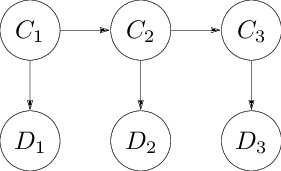
\includegraphics[width=0.25\textwidth]{media/car.jpeg}
\end{center}

The distribution over the initial car distribution is uniform; that is, for each
value $c_1 \in \{0, 1\}$:
\[ p(c_1) = 0.5. \]

The following local conditional distribution governs the movement of the car
(with probability $\epsilon$, the car moves). For each $t \in \{2, 3\}$:
\[ p(c_t \mid c_{t-1}) =
\begin{cases}
  \epsilon & \text{if $c_t \neq c_{t-1}$} \\
  1-\epsilon & \text{if $c_t = c_{t-1}$}.
\end{cases}
\]

The following local conditional distribution governs the noise in the sensor
reading (with probability $\eta$, the sensor reports the {\em wrong} position).
For each $t \in \{1, 2, 3\}$:
\[
p(d_t \mid c_t) =
\begin{cases}
  \eta & \text{if $d_t \neq c_t$} \\
  1-\eta & \text{if $d_t = c_t$}.
\end{cases}
\]

Below, you will be asked to find the posterior distribution for the car's
position at the second time step ($C_2$) given different sensor readings.

{\bf Important}:

For the following computations, try to follow the general strategy described in
lecture (marginalize non-ancestral variables, condition, and perform variable
elimination). Try to delay normalization until the very end. You'll get more
insight than trying to chug through lots of equations.

\begin{enumerate}

  \input{01-bayesian-network-basics/01-second-timestep}

  \input{01-bayesian-network-basics/02-third-timestep}

  \input{01-bayesian-network-basics/03-interpret}

\end{enumerate}
